% Draft Fig.: management architecture -- three loops at three time scales and
% where each would run in a deployment. Build: pdflatex fig_arch.tex
\documentclass[tikz,border=3pt]{standalone}
\usepackage{times}
\usetikzlibrary{arrows.meta,positioning,fit,calc,backgrounds}
\begin{document}
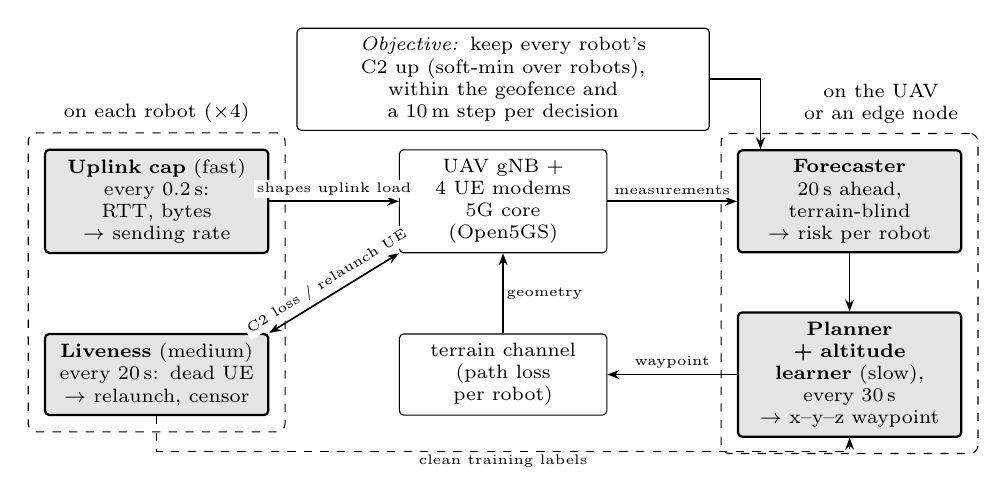
\begin{tikzpicture}[font=\scriptsize,
  loop/.style={draw, thick, rounded corners=1.5pt, fill=black!10, align=center, minimum height=10mm, text width=26mm},
  sys/.style={draw, rounded corners=1.5pt, align=center, minimum height=10mm, text width=24mm},
  zone/.style={draw, dashed, rounded corners=3pt, inner sep=2mm},
  lab/.style={font=\tiny, fill=white, inner sep=1pt},
  ar/.style={-{Stealth[length=1.5mm]}, semithick}]
\node[sys] (cell) at (0,0) {UAV gNB + 4 UE modems\\5G core (Open5GS)};
\node[sys] (chan) at (0,-2.2) {terrain channel\\(path loss per robot)};
\node[loop] (cap)  at (-4.4,0)    {\textbf{Uplink cap} (fast)\\every 0.2\,s: RTT, bytes\\$\to$ sending rate};
\node[loop] (live) at (-4.4,-2.2) {\textbf{Liveness} (medium)\\every 20\,s: dead UE\\$\to$ relaunch, censor};
\node[loop] (fc)   at (4.4,0)     {\textbf{Forecaster}\\20\,s ahead, terrain-blind\\$\to$ risk per robot};
\node[loop] (pl)   at (4.4,-2.2)  {\textbf{Planner + altitude}\\\textbf{learner} (slow), every 30\,s\\$\to$ x--y--z waypoint};
\node[draw, rounded corners=1.5pt, align=center, text width=50mm] (obj) at (0,1.55)
  {\textit{Objective:} keep every robot's C2 up (soft-min over robots),\\within the geofence and a 10\,m step per decision};
\begin{scope}[on background layer]
\node[zone, fit=(cap)(live), label={[font=\scriptsize]above:on each robot ($\times$4)}] {};
\node[zone, fit=(fc)(pl), label={[font=\scriptsize, align=center, xshift=4mm]above:on the UAV\\or an edge node}] {};
\end{scope}
\draw[ar] (cap) -- node[lab, above=1pt]{shapes uplink load} (cell);
\draw[{Stealth[length=1.5mm]}-{Stealth[length=1.5mm]}, semithick] (live.north east) -- node[lab, sloped, above=1pt]{C2 loss / relaunch UE} (cell.south west);
\draw[ar] (cell) -- node[lab, above=1pt]{measurements} (fc);
\draw[ar] (fc) -- (pl);
\draw[ar] (pl) -- node[lab, above=1pt]{waypoint} (chan);
\draw[ar] (chan) -- node[lab, right]{geometry} (cell);
\draw[ar, dashed] (live.south) -- ++(0,-0.45) -| node[lab, pos=0.25, below]{clean training labels} (pl.south);
\draw[ar] (obj.east) -| ([xshift=3mm]fc.north west);
\end{tikzpicture}
\end{document}
